\documentclass{article}

\usepackage[margin=1in]{geometry}
\usepackage{parskip}
\usepackage{datetime}
\usepackage{url}
\usepackage{hyperref}
\usepackage[utf8]{inputenc}
\usepackage{graphicx}
\usepackage{tikz}
\usepackage{listings}

\lstset{
    basicstyle=\ttfamily
}

\newdateformat{required}{\twodigit{\THEMONTH}/\twodigit{\THEDAY}/\THEYEAR}
\raggedbottom

\begin{document}

\begin{titlepage}
    \begin{center}
        \begin{huge}
        House in Your Head \\[1cm]
        Team G1-FrigidWaters \\[2.2cm]
        { \bfseries System Design Specification } \\[1cm]
        Cycle \# 2\\[2.2cm]
        Date: \required\today\\[1cm]
        \end{huge}
    \end{center}
    \null \vfill
    \begin{large}
        Team Members: \\[0.5cm]
        Name: Samuel Bever\\[0.5cm]
        Name: Michael Conway\\[0.5cm]
        Name: Joseph Muoio\\[0.5cm]
        Name: Kyle Patron\\[0.5cm]
        Name: Kevin Zakszewski
    \end{large}
\end{titlepage}
\section*{\centering Table of Contents}
\makeatletter
\@starttoc{toc}
\newcommand{\hsubsubsection}{
\@startsection{subsubsection}{3}{\z@}%
                                     {-3.25ex\@plus -1ex \@minus -.2ex}%
                                     {-1.5ex \@plus -.2ex}% Formerly 1.5ex \@plus .2ex
                                     {R\normalfont\normalsize}}
\newcommand{\hparagraph}{
\@startsection{paragraph}{4}{\z@}%
                                     {-3.25ex\@plus -1ex \@minus -.2ex}%
                                     {-1.5ex \@plus -.2ex}% Formerly 1.5ex \@plus .2ex
                                     {R\normalfont\normalsize}}
\newcommand{\hsubparagraph}{
\@startsection{subparagraph}{5}{\z@}%
                                     {-3.25ex\@plus -1ex \@minus -.2ex}%
                                     {-1.5ex \@plus -.2ex}% Formerly 1.5ex \@plus .2ex
                                     {R\normalfont\normalsize}}
\setcounter{secnumdepth}{5}
\makeatother
\newpage
 

\section{Introduction}

\subsection{Purpose}
The purpose of this document is to describe the data, interface, architectural, and component-level design for our project. The architectural section will go over the modules and components, their relationship, and will describe the structure of the system as a whole. The interface section contains more detail on the system's user interface, data interface,  and the programming interface. Finally, in the remaining portion of this document, any other design details or relationships will be laid out.

\subsection{Scope}

This system is intended to be a Brain Computer Interface that will act as a bridge between data received from the Emotiv device and a home automation system. The system on the end of the Emotiv device and the home automation system are a a bit like black boxes. We are more concerned with taking the data, interpreting it correctly and triggering the correct actions in the home automation system. The functionality of the other two systems are out of our scope. 

\subsection{Definitions, Acronyms, and Abbreviations}
\begin{description}
    \item[EEG] Can refer to:
        \begin{itemize}
            \item Electroencephalography - Recording of the brain's electrical
                activity.
	        \item Electroencephalogram - The device that is used to record the
	            brain's electrical activity.
        \end{itemize}
    \item[Emotiv] The electroencephalogram hardware device, created by Emotiv
        Limited, used to read the user's brain activity (EEG).
    \item[Brain Computer Interface (BCI)] The class of devices that the Emotiv
        belongs to.
    \item[Amyotrophic Lateral Sclerosis (ALS)] A neurodegenerative disorder
        that our target users suffer from. The main characteristics of ALS
        that we are concerned with in the scope of this project are the
        limited movement and mobility to complete paralysis.
    \item[Application Program Interface (API)] Software level functions which
        allow other parts of the system (or external systems) to interact and 
        share data.
\end{description}


\subsection{Overview}
The next section is the architectural description. In that section there is
an overview of components and modules, a description of the system
structure, and component relationships. In the third section, the system
interfaces are laid out. This contains the user interface, data interface,
and programming interface. The fourth section is composed of subsections
describing the detailed design of the system. The fifth section looks at the
relationship of the system to other products. The sixth section details the
design decisions and tradeoffs of the system. The final section shows some
rough psuedocode of the main components of the system.

\subsection{Requirements Traceability Matrix}
\begin{tabular}{ | l | l | l | l | l | l | l | l | l | l |}
\hline
\textbf{Requirements Identifiers} & SR105 & SR110 & SR115 & SR120 & SR205 & SR210 & SR215 & SR220 & SR225 \\ \hline
\textbf{1.0} & X &  &  &  & X & X &  &  & \\ \hline
\textbf{2.0} &  &  &  & &  &  &  &  & X \\ \hline
\textbf{2.1} &  &  &  & &  &  &  &  & X \\ \hline
\textbf{2.2} &  &  &  & &  &  &  &  & X \\ \hline
\textbf{3.0} &  &  &  &  & X &  & X & X & \\ \hline
\textbf{4.0} &  & X & X & X &  &  &  &  & \\ \hline
\end{tabular}

\newpage

\section{Architectural Description}

\subsection{Overview of modules / components}

\begin{figure}[h!]
    \centering
    \resizebox{\textwidth}{!}{
        \input{dfd-context.pgf}
    }
    \caption{Context diagram.}
    \label{fig:dfd-context}
\end{figure}

% TODO describe
\autoref{fig:dfd-context}

\begin{figure}[h!]
    \centering
    \resizebox{\textwidth}{!}{
        \input{dfd-0.pgf}
    }
    \caption{Level 0 DFD.}
    \label{fig:dfd-0}
\end{figure}

\autoref{fig:dfd-0} is a broken-out version of \autoref{fig:dfd-context}. The
three main components of the system are the EEG Processing component, which
processes signals from the Emotiv device; the GUI/Control layer, which
displays the menu to the Patient and translates input from EEG Processing into
menu selections; and the HAS Interface, which receives commands from the
GUI/Control layer and passes them to the available Insteon devices.

\begin{figure}[h!]
    \centering
    \resizebox{\textwidth}{!}{
        \input{dfd-1.pgf}
    }
    \caption{Level 1 DFD of the EEG Processing System (1).}
    \label{fig:dfd-1}
\end{figure}

\begin{figure}[h!]
    \centering
    \resizebox{\textwidth}{!}{
        \input{dfd-2.pgf}
    }
    \caption{Level 1 DFD of the User Interface (2).}
    \label{fig:dfd-2}
\end{figure}

\begin{figure}[h!]
    \centering
    \resizebox{\textwidth}{!}{
        \input{dfd-3.pgf}
    }
    \caption{Level 1 DFD of the HAS Interface (3).}
    \label{fig:dfd-3}
\end{figure}

% TODO more?
\autoref{fig:dfd-3} describes the interaction of components within the HAS
Interface.

\subsection{Structure and relationships}
% FIXME Would be nice to section according to the DFD, but requires more plumbing

\subsubsection{Component 1: EEG Processing}
This component receives input from the patient (via the Emotive device) and
configuration commands from the control layer. It then returns the current
state the user is in (concentrating/not concentrating) and stores data
during from the training process.

\subsubsection{Component 1.1: Data Filter}
This performs simple filtering on the data from the Emotiv device. One of
the most necessary filters for testing requires that the software ignore all
EEG data if the accelerometer senses movement, since movement disrupts the
signals. It will also provide simple filtering that will remove any data
that has too much noise in it to be useful. This component then passes the
data to the main EEG processor.

\subsubsection{Component 1.2: EEG Processor}
This component takes in the filtered EEG data from the Data Filter (1.1) and the current configuration data from the Control Layer(2). Using this, it performs two actions. First, if it is in training mode, it analyzes the EEG and detects patterns corresponding to the time the user was trying to select an option. If it succeeds, it puts the data about the user and that trained state into the Training Data Storage (1.3). If we are currently running, the EEG Processor retrieves data from the Training Data Store matching the current user. It compares the trained states to the current EEG data. If it gets a match, it returns the corresponding state. Otherwise, it returns the neutral state.

\subsubsection{Component 1.3: Training Data Storage}
This system stores trained states by user. It contains the observed amplitude, change in amplitude, frequency, and change in frequency for each electrode during the training process. It is written to during the training process and is queried while running to see if the current data matches any stored states.

\subsubsection{Component 2: GUI/Control Layer}
% TODO
This component receives input from the EEG processing (1), updates the screen, and sends high level commands to the HAS Interface (3). 

\subsubsection{Component 2.1: UI Cycle Routine}
The UI Cycle Routine cycles through all of the available Interactive State Pages (2.3) one by one, and receives input from the EEG processing to select one. 

\subsubsection{Component 2.2: Configuration Routine}
The Configuration Routine is responsible for configuring the device for the user's session. This runs before going to the UI Cycle Routine (2.1) and communicates the results to the EEG Processing (1). 

\subsubsection{Component 2.3: Interactive State Pages}
The Interactive State Pages have one for each insteon device connected to the system. This page takes input from the EEG processing module (1). Any selections are sent as high level commands to the Device Manager (3).

\subsubsection{Component 3: HAS Interface}
This component translates the control signals generated in the GUI/Control
Layer (2) and uses them to control the house via the Insteon PowerLinc Modem,
attached via USB.

\subsubsection{Component 3.1: Device Manager}
The device manager manages the list of available Devices (3.2) and publishes
it to the GUI/Control Layer (2). It also handles device discovery and
configuration, as well as configuration persistence (Device Config File,
D3.4).

\subsubsection{Component 3.2: Devices}
Devices define the available home automation devices and the user-selectable
actions that can be performed on each. They are registered with and provide
status updates to the Device Manager (3.1); receive commands from the
GUI/Control Layer (2); and fulfill these commands by composing lower-level
commands made avaiable by the Drivers (3.3).

\subsubsection{Component 3.3: Drivers}
Drivers wrap the low-level serial interface to Insteon devices through the
PowerLinc Modem and provide the available simple operations and status updates
to Devices (3.2).

\subsubsection{Component D3.4: Device Config File}
The configuration of available devices is persisted per-installation in a
local file in JSON format.

\newpage

\section{Interface Description}

\subsection{User Interface}

The user interface of the system is intended to be simple because most of
the data received in the system, as well as the choices made by the user,
are either yes or no decisions (i.e. binary data). When the application is
started, the user will first be presented with the configuration screen. A
prompt to configure the "accept" thought is displayed. After the
configuration timer has elapsed, the application advances to test the
configuration. The user is promped to think their accept thought to
continue. If there is an error, they will be redirected to an error screen
and the application will retry the configuration process. Once the
configuration process is successfully complete, the application moves to the
application selection screen. 

\begin{figure}[h!]
	
  \centering
    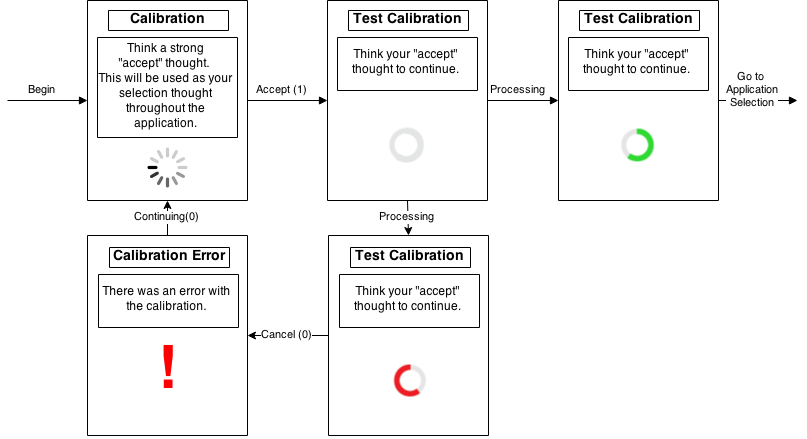
\includegraphics[width=0.7\textwidth]{ConfigurationUI}
   \caption{Sample Configuration interface}
   \label{fig:ui}
\end{figure}

At the application selection screen, the user will cycle through the options
of the objects that they can interact with in the home automation system.
This is also the screen where the user decides which object they want to
interact with. When an object is chosen, the user will be directed to the
interactive state screen for the selected object. This screen handles the
changing of the state of the object the user selects. From this screen the
user can either change the state or return to the previous screen (the first
type where the users cycle through the options). These three types of UI
screens will make up the majority of the user interaction in the system.
These designs will be modified or extra user interface designs will be
implemented as necessary. 

\begin{figure}[h!]
	
  \centering
    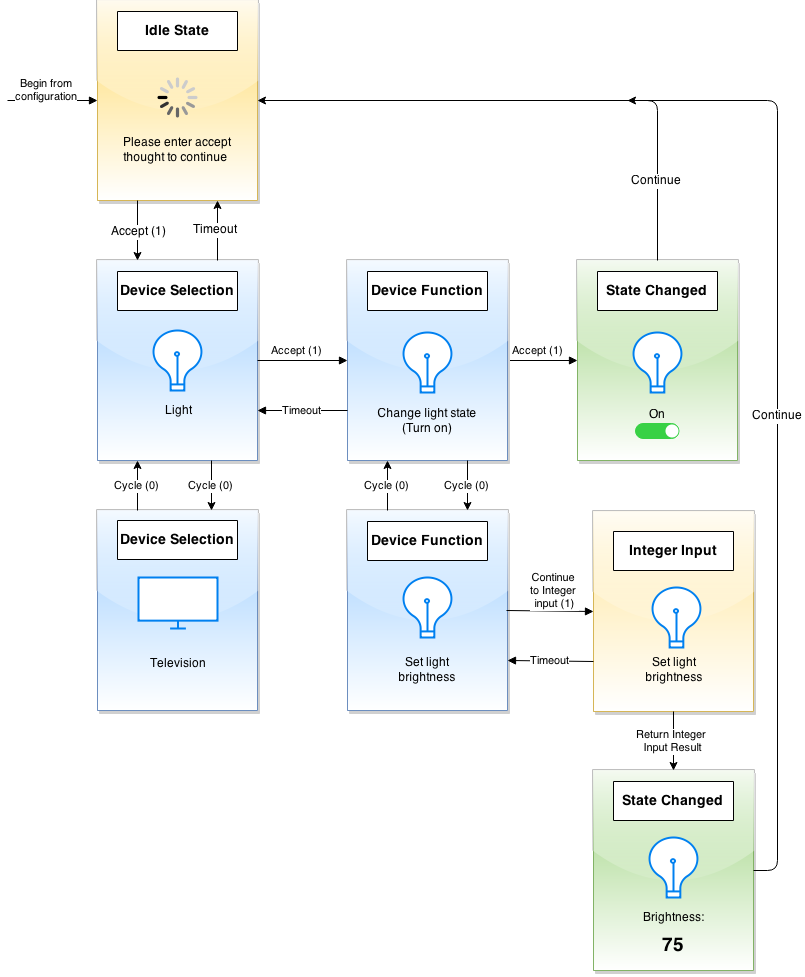
\includegraphics[width=0.7\textwidth]{ApplicationUI}
   \caption{Sample User interface}
   \label{fig:ui}
\end{figure}

\subsection{Data Interface}
\begin{figure}[h!]

  \centering
  \resizebox{\textwidth}{!}{
        \input{erd.pgf}
    }
   \caption{ERD}
   	\label{fig:erd}
\end{figure}

The data flowing into our program will consist of a tuple of floats,
representing the EEG data at any given time. There will also be a JSON blob
that stores the parameters that should be used in signal extraction. The
output will be in the form of calling methods of the home automation system.
\autoref{fig:erd} shows the internal representation of the user, house and
state. This consists of a binary tree of UI structures, which may or may not
reference a device to call the method of.
% XXX Huh?

\subsection{Programming Interface} 
There is no need for a programming interface because it is a generic, self-contained system.

\newpage

\section{Detailed Design}

\subsection{Component Template Description}

The design entities include the following:

\begin{tabular}{ | l |  p{13.3cm} |}
\hline
\textbf{Type} & The type of Entity. This could be one of the following: Module, or Data Store. \\ \hline
\textbf{Purpose} & The reason the entity exists.  \\ \hline
\textbf{Function} & What the entity does. \\ \hline
\textbf{Subordinates} & All entities that compose the entity. \\ \hline
\textbf{Dependencies} & The relationship of the entity to others. \\ \hline
\textbf{Interface} & How this entity interacts with other entities \\ \hline
\textbf{Resources} & External elements used by the system. \\ \hline
\textbf{Processing} & The algorithm used for the entity. \\ \hline
\textbf{Data} & View ERD for the data. \\ \hline
\end{tabular}

\subsection{Design Entities}

\subsubsection*{1.0 - EEG Interpreter}
\begin{tabular}{ | l |  p{13.3cm} |}
\hline
\textbf{Type} & Module \\ \hline
\textbf{Purpose} & Determines if the current brain scan information matches the trained data \\ \hline
\textbf{Function} & Looks at the current EEG information coming from the user's brainwaves and compares this to the data that was trained to see if it matches one of the trained classes. \\ \hline
\textbf{Subordinates} & None \\ \hline
\textbf{Dependencies} & Relies on Training datastore (2.2). There needs to be trained models to compare the stream of data to. \\ \hline
\textbf{Interface} & The EEG Interpreter will have an API that can be polled by other components. \\ \hline
\textbf{Resources} & The EEG information comes from the emotive device. \\ \hline
\textbf{Processing} & Each entry in the Training datastore will have a set of changes or values that will constitute entry into that state. This module will continually analyze the incoming EEG data to see if the changes or the current values match the values stored in the datastore. There will be four values that will be analyzed for each electrode of the EEG. They will be amplitude, change in amplitude, frequency, and change in frequency. If the values for each of those metrics are close to the trained data, then we will say that we are in that state.\\ \hline
\textbf{Data} & See ERD in Section 3 \\ \hline
\end{tabular}

\subsubsection*{2.0 - Training Module}
\begin{tabular}{ | l |  p{13.3cm} |}
\hline
\textbf{Type} & Module \\ \hline
\textbf{Purpose} & Trains a model for the current user for each state. \\ \hline
\textbf{Function} & Delegates to state trainers for each state that needs to be trained for the current user. Then stores this in the Training Datastore (2.2). \\ \hline
\textbf{Subordinates} & State Trainer (2.1). Every state that needs to be trained will be trained through a specific state trainer for that state. \\ \hline
\textbf{Dependencies} & Training Datastore (2.2). This is needed to save the trained models. \\ \hline
\textbf{Interface} & None \\ \hline
\textbf{Resources} & None \\ \hline
\textbf{Processing} & For each State Trainer (2.1) that is untrained, train the state model for that trainer. Then, save the results to the Training Datastore (2.2). Training will take place by asking the user to think at the trigger at certain times. The amplitude, frequency, change in amplitude and change in frequency will be evaluated at those points and will constitute the state being trained. \\ \hline
\textbf{Data} & See ERD in Section 3 \\ \hline
\end{tabular}

\subsubsection*{2.1 - State Trainer}
\begin{tabular}{ | l |  p{13.3cm} |}
\hline
\textbf{Type} & Module \\ \hline
\textbf{Purpose} & Trains a model for a single state. \\ \hline
\textbf{Function} & Trains a model for a specific state. Each state trainer trains on one state, so there will be a State Trainer for the resting state, active state, and any other states deemed necessary in the future. \\ \hline
\textbf{Subordinates} & None \\ \hline
\textbf{Dependencies} & GUI Module (3.0). To train a model, interaction with the user of the system is required. This is done through a Graphic User Interface.  \\ \hline
\textbf{Interface} & None \\ \hline
\textbf{Resources} & None \\ \hline
\textbf{Processing} & Interact with the user on the screen until a model is built based on the user's personal EEG. \\ \hline
\textbf{Data} & See ERD in Section 3 \\ \hline
\end{tabular}

\subsubsection*{2.2 - Training Datastore}
\begin{tabular}{ | l |  p{13.3cm} |}
\hline
\textbf{Type} & Data store \\ \hline
\textbf{Purpose} & Holds the trained data for the current user. \\ \hline
\textbf{Function} & Holds all the trained states for the current user of the system. This includes the resting state and the active state at a minimum. Other states will be explored in the future. \\ \hline
\textbf{Subordinates} & None \\ \hline
\textbf{Dependencies} & None \\ \hline
\textbf{Interface} & The training datastore will have an API that allows read and write access to it. \\ \hline
\textbf{Resources} & May need hard disk space if it will be saved permanently.  \\ \hline
\textbf{Processing} & The currently loaded user's data will be the only data retrieved. Loading from disk and saving to disk is allowed. The datastore will store the amplitude, frequency, change in frequency, and change in amplitude for each state.\\ \hline
\textbf{Data} & See ERD in Section 3 \\ \hline
\end{tabular}

\subsubsection*{3.0 - GUI Module}
\begin{tabular}{ | l |  p{13.3cm} |}
\hline
\textbf{Type} & Module \\ \hline
\textbf{Purpose} & Hands output from the system to an external monitor. \\ \hline
\textbf{Function} & All interaction with the user is through an external monitor. This system handles all output to the screen. \\ \hline
\textbf{Subordinates} & None \\ \hline
\textbf{Dependencies} & None \\ \hline
\textbf{Interface} & There will be a writer API to allow other parts of the system to output to the screen. \\ \hline
\textbf{Resources} & External Monitor \\ \hline
\textbf{Processing} & The GUI module will wait until given something to write to the screen. When it is given a request, it will write that request to the screen. \\ \hline
\textbf{Data} & See ERD in Section 3 \\ \hline
\end{tabular}

\subsection*{4.0 - Home Automation Interface}
\begin{tabular}{ | l |  p{13.3cm} |}
\hline
\textbf{Type} & Module \\ \hline
\textbf{Purpose} & Interfaces with external home automation controls. \\ \hline
\textbf{Function} & Manages the system's interface with external home
automation controls. This includes providing the rest of the system with
information about available controls, maintaining any necessary state, and
processing requests to manipulate the home via the controls. \\ \hline
\textbf{Subordinates} & None \\ \hline
\textbf{Dependencies} & None \\ \hline
\textbf{Interface} & The interface will support querying for information about
available home controls and to manipulate the home via the controls. \\ \hline
\textbf{Resources} & Home automation system controls \\ \hline
\textbf{Processing} & The module will query control state as necessary and
reject requests that are not valid in the current state. \\ \hline
\textbf{Data} & See ERD in Section 3 \\ \hline
\end{tabular}

\newpage

\section{Reuse and Relationships to other Products}
\label{sec:ReuseRel}

There has been previous related work done with the Emotiv device by related
researchers. However, their interface was unappealing and their code messy. It
may be referenced to help understand the Emotiv device, but it will not be
reused directly.

There are very few commercially available BCI devices, and often there is no
software available for them. The few that do exist are prohibitively
expensive. Having the Emotiv available at a reasonable price will improve the
quality of life for many ALS patients.

\section{Design decisions and tradeoffs}

The first design decision was what type of interface to use.  The options
available were EEG sensor devices, eye movement trackers, and facial muscle
detecting devices. EEG sensors seemed the best fit as they will work for all
ALS patients, including those that are ``locked in.'' A locked-in patient
may be unable to use their facial muscles or move their eyes. In addition,
this means that a patient will not have to relearn how to use the system
with new interfaces as their disease progresses.

Another design decision was what device should be used to best assist ALS
patients. As noted in \autoref{sec:ReuseRel}, there already exist devices with
similar functionality, but they are much more expensive. The Emotiv is \$500,
which is affordable when compared to its alternatives. The Emotiv is capable
of detecting up to four thoughts plus a neutral state, which provides enough
flexibility to design features in a number of ways.

Given this flexiblity, deciding how users should interface with the system was
the next step. Previous user reviews indicated that training the Emotiv to
recognize multiple thoughts was challenging, suggesting that a binary
interface would be the most useful. On the other hand, an interface that uses
a larger substantial branching would enable users to navigate it much more
quickly. The binary interface was chosen in order to maximize ease-of-use.

% TODO Is this a design decision, or was it made as a part of requirements?
The main purpose of the interface, home automation, was decided upon because
it allows patients to regain capabilities that they have lost. It also
serves as a proof of concept for interfacing with nontrivial systems.

\newpage

\section{Psuedocode for components}

\subsection*{1.0 - EEG Interpreter}

\begin{lstlisting}
repeat forever:
    monitor EEG
    if EEG in a trained state:
        notify all registered listeners of new data
        % TODO OR call all registered callbacks
\end{lstlisting}

\subsection*{2.0 - Training Module}

Upon training request:

\begin{lstlisting}
for each untrained State Trainer:
    run the trainer
save results to Training Datastore
\end{lstlisting}

Each State Trainer:

\begin{lstlisting}
repeat until trained:
    display prompt
    collect data from EEG Interpreter
    update training parameters
\end{lstlisting}

\subsection*{3.0 - GUI Module}

Upon menu display request:
\begin{lstlisting}
% TODO OPTION A
display menu
for each menu option:
    register callback for corresponding state in EEG Interpreter
% TODO OPTION B
display menu
register self as EEG Interpreter listener for necessary states
upon state notification, perform action
\end{lstlisting}

\subsection*{4.0 - Home Automation Interface}

Upon receiving a control request:

\begin{lstlisting}
if request is valid:
    perform action
else:
    report error
\end{lstlisting}

\newpage

\section*{\centering Table of Contributions}
\begin{tabular}{| l | l | l | l |}
    \hline
     & Section & Writing & Editing \\
    \hline \hline
		1 & 2, 3.2 & Kyle Patron & Michael Conway \\ \hline
		2 & 1.5, 4 & Joe Muoio & Kyle Patron \\ \hline
		3 & 5, 6 & Sam Bever &  Kevin Zakszewski \\ \hline
		4 & 7 & Michael Conway &  Sam Bever \\ \hline
		5 & 1, 3.1 & Kevin Zakszewski &  Joe Muoio \\ \hline
\end{tabular}
\newpage
\noindent I certify that:
\begin{itemize}
\item This paper/project/exam is entirely my own work.
\item I have not quoted the words of any other person from a printed source or a website without indicating what has been quoted and providing an appropriate citation.
\item I have not submitted this paper / project to satisfy the requirements of any other course.
\end{itemize}

\vspace{1cm}
\noindent\makebox[\textwidth][l]{
Signature:
\makebox[5cm][l] {\underline{Samuel Bever}} 
\ \ Date:
\makebox[4cm][l] {\underline{\required\today}} 
}


\vspace{0.5cm}
\noindent\makebox[\textwidth][l]{
Signature:
\makebox[5cm][l] {\underline{Michael Conway}} 
\ \ Date:
\makebox[4cm][l] {\underline{\required\today}} 
}

\vspace{0.5cm}
\noindent\makebox[\textwidth][l]{
Signature:
\makebox[5cm][l] {\underline{Joe Muoio}} 
\ \ Date:
\makebox[4cm][l] {\underline{\required\today}} 
}

\vspace{0.5cm}
\noindent\makebox[\textwidth][l]{
Signature:
\makebox[5cm][l] {\underline{Kyle Patron}} 
\ \ Date:
\makebox[4cm][l] {\underline{\required\today}} 
}

\vspace{0.5cm}
\noindent\makebox[\textwidth][l]{
Signature:
\makebox[5cm][l] {\underline{Kevin Zakszewski}} 
\ \ Date:
\makebox[4cm][l] {\underline{\required\today}} 
}

\vspace{\fill}
\subsection*{Grading}
The grade is given on the basis of quality, clarity, presentation, completeness, and writing of each section in the report. This is the grade of the group. Individual grades will be assigned at the end of the term when peer reviews are collected.
\end{document}
